\chapter{Compararea modelelor finale}

În final, antrenăm fiecare tip de model cu hiperparametrii optimi găsiţi 
folosind setul de validare şi folosim setul de testare pentru a evalua
imparţial modelele finale.

\begin{table}[H]
    \centering
    \begin{tabularx}{\textwidth}{
        |X
        |X
        |X
        |X
        |X|
    }
    \hline
    {Model} & {Accuracy} & {Precision} & {Recall} & {F1 Score} \\
    \hline
    \rowcolor{gray!20} \text{OCSVM} & 0.8913 & 0.0577 & 0.8823 & 0.1080 \\
    \text{KDE} & 0.8911 & 0.0575 & 0.8823 & 0.1078 \\
    \rowcolor{gray!20} \text{GMM} & 0.8728 & 0.0554 & 0.8455 & 0.1058 \\
    \hline
    \end{tabularx}
    \caption{Performanţa fiecărui model pe setul de testare}
\end{table}

Toate cele 3 modele au o performanţă similară, Gaussian Mixture Model fiind foarte puţin mai slab
decât One Class SVM şi Kernel Density Estimation care sunt aproximativ egale din punct de vedere al
metricilor de evaluare. Precision este scăzut şi prin urmare şi 
f1 score este scăzut. În schimb, recall are o valoare ridicată pentru toate modelele. Acest 
fapt ne arată că detectăm aproape toate anomaliile, dar în acelaşi timp, semnalăm un număr 
mare de tranzacţii obişnuite ca fiind frauduloase. Acest lucru poate deveni un inconvenient 
pentru client în cazul în care tranzacţia este anulată ca urmare a raportării incorecte.

One class SVM este modelul cu valorile cele mai mari pentru toate metricile, dar este 
şi un model mai complex faţă de celelalte 2 tehnici clasice de estimare a densităţii. Totuşi, 
este de menţionat faptul că modelul de Gaussian Mixture Model a necesitat doar 3 minute pentru
antrenare şi prezicere a etichetelor, dar a produs rezultate aproape la fel de bune precum
One class SVM şi Kernel Density Estimation care au avut nevoie de mai mult de o oră şi jumătate,
respectiv 4 ore şi jumătate, cel din urmă neavând o performanţă cu mult mai ridicată în raport 
cu complexitatea de timp.

Ilustrăm şi ROC Curve alături de metrica AUC pentru modelele finale. Cu cât graficul 
tinde să se lipească de colţul stânga sus, cu atât aria de sub grafic creşte rezultând 
într-o performanţă mai bună. Linia punctată pe diagonală 
din fiecare diagramă reprezintă graficul produs de clasificatorul aleatoriu şi are rolul
de a marca marginea inferioară a performanţei faţă de această metrică. De asemenea, este 
de menţionat că dacă graficul se află sub linia diagonală, atunci am trage concluzia că
algoritmul nostru este inutil. Totuşi, putem inversa clasa negativă cu cea pozitivă şi 
astfel obţinem simetricul graficului faţă de diagonală care acum, evident, se află deasupra
liniei. Prin urmare, distanţa între grafic şi linie este o măsură mai relevantă decât poziţia
relativă. Se presupune că operaţia de aplicare a simetricului este folosită unde este cazul 
pentru diagramele de mai jos.

ROC Curve are nevoie ori de probabilităţi ori de valori ce exprimă încrederea pentru fiecare 
prezicere, fără aplicarea vreunui prag. Kernel Density Esimation şi Gaussian Mixture Model 
produc deja probabilităţi, pe când One Class SVM nu produce decât distanţa faţă de hiperplanul
de separare. Totuşi, vom folosi un truc pentru a transforma rezultatele OCSVM în valori 
de încredere \cite{stackoverflow-auc}. Înlocuim fiecare valoare cu valoarea respectivă scăzută din valoarea maximă
dată de funcţia de decizie după cum urmează:

$$y_{score} = MAX - f(y)$$
unde 

\begin{itemize}
    \item $y_{score}$ este valoarea folosită pentru ROC Curve
    \item $MAX$ este $\max_{i=1}^{n} f(y_{i})$ pentru $n$ observaţii
    \item $f$ este funcţia de decizie 
\end{itemize}

Astfel, putem compara modelele finale folosind şi metrica AUC. Clasamentul este acelaşi şi aici,
cu One Class SVM fiind cel mai performant, urmat de Kernel Density Estimation, iar Gaussian Mixture
Model la coadă.

\begin{figure}[p] % Use a separate page for the figure
    \begin{minipage}[t]{0.5\textwidth}
        \vspace{0pt}
        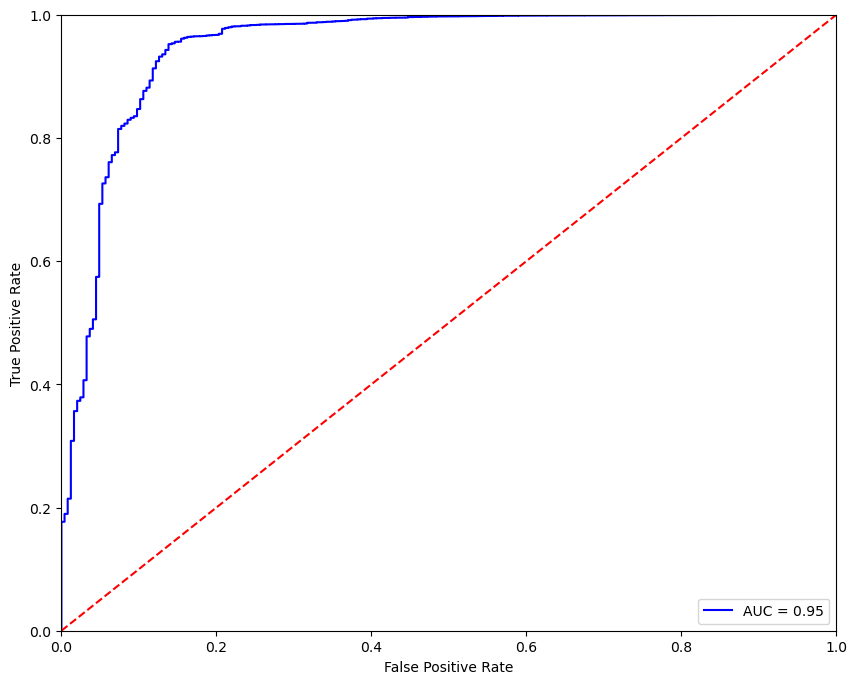
\includegraphics[width=\textwidth]{images/ocsvm-roc.png}
        \caption{ROC Curve OCSVM}
    \end{minipage}
    \hfill
    \begin{minipage}[t]{0.5\textwidth}
        \vspace{0pt}
        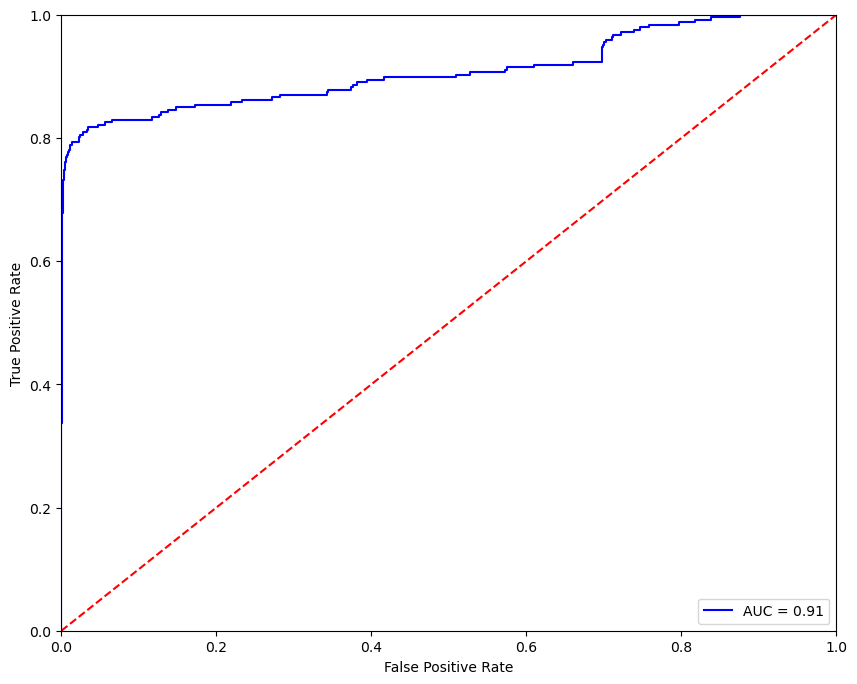
\includegraphics[width=\textwidth]{images/gmm-roc.png}
        \caption{ROC Curve GMM}
    \end{minipage}
    
    \begin{minipage}[t]{1\textwidth}
       \centering
        
        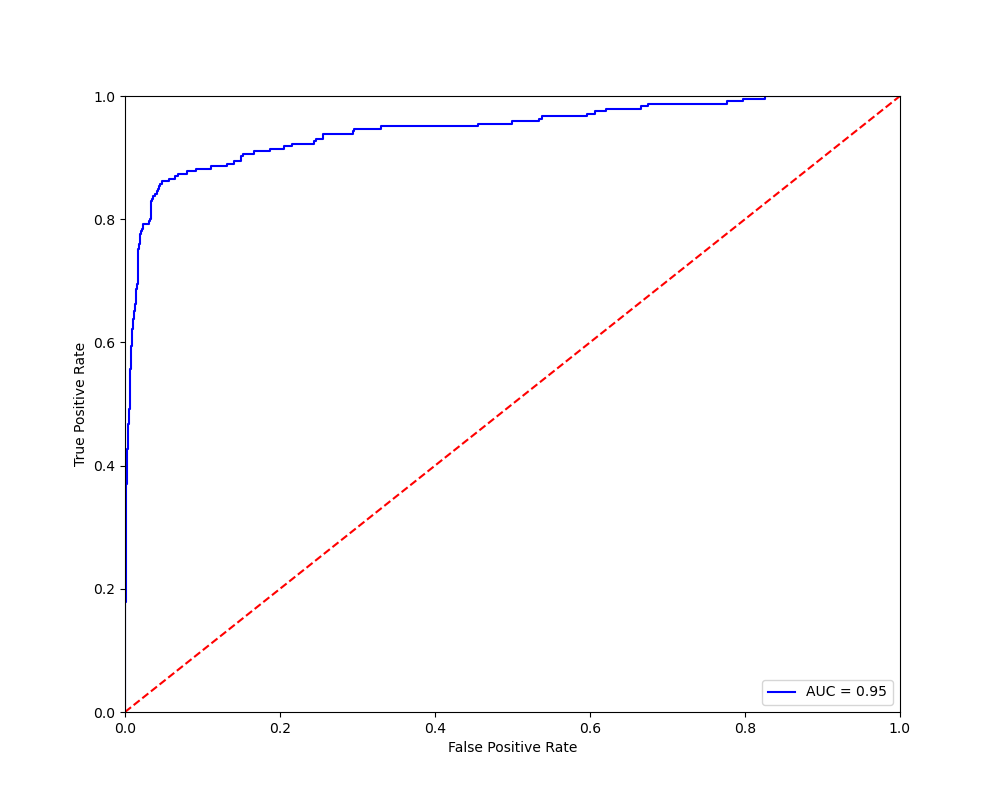
\includegraphics[width=\textwidth]{images/kde-roc.png}
        \caption{ROC Curve KDE} 
    \end{minipage}
    
\end{figure}

\noindent